
\section{Loss function optimization}

%%%%%%%%%%%%%%%%%%%%%%%%%%%%%%%%%%%%%%%%%%%%%%%%%%%%%%
%%%%%%%%%%%%%%%%%%%%%%%%%%%%%%%%%%%%%%%%%%%%%%%%%%%%%%
%%%%%%%%%%%%%%%%%%%%%%%%%%%%%%%%%%%%%%%%%%%%%%%%%%%%%%

For this section, I use definitions from \cite{nocedal2006numerical} and \cite{1606.04838}.


In statistical learning, one usually wants to find the parameters that minimize a loss function, which almost always has to do with the error of the model we're using. In many cases, as in linear regression, using the first and second order conditions, we can find a closed formula to find the parameters. But there are many other cases in which this isn't possible, that's when numerical optimization comes in. 
The general problem of unrestricted optimization is

\begin{equation}
  \min_{\theta \in \mathbb{R}^p} L(\theta).
\end{equation}

For statistical learning, $L$ is usually a convex loss function such as quadratic loss, and $\theta$ is a parameter or vector of parameters. Generally, numerical optimization algorithms are iterative. A solution is a vector $\theta^*$ called local minimizer, which makes the function $L$ to be minimized in a neighbourhood around $\theta^*$. Formally, a vector $\theta^*$ is a local minimizer if there exists a neighbourhood $\mathcal{N}$ of $\theta^*$ such that $L(\theta^*) \leq L(\theta)$ for all $\theta \in \mathcal{N}$.

In numerical optimization, we make use of the sufficient second order conditions. Suppose that the Hessian matrix $\nabla^2 L$ is continuous in an open neighbourhood of $\theta^*$, that the gradient $\nabla L(\theta^*) = 0$ and that $\nabla^2 L(\theta^*)$ is positive definite; then $\theta^*$ is a local minimizer of $L$.

This is basic calculus, but it provides the base of numerical optimization algorithms. In general, all algorithms search for a point $\theta^*$ such that $\nabla L(\theta^*) = 0$. 



\subsection{Gradient descent (GD)}

Gradient descent is an algorithm that belongs to a family called *line search algorithms*. In each iteration, thee algorithms search for a direction in which to go and then update the current value in accordance to that direction. That is, in the $k$-th iteration, we have a value $\theta_k$, and we look for a direction $p_k$ to update to a new value $\theta_{k+1} = \theta_k + \alpha_k p_k$, where $\alpha_k > 0$ is the 'distance' that the algorithm moves toward direction $p_k$, and is called *step length*. Once that the value of the parameter is updated, we find a new direction in which to move forward and then update the parameter value again. This is done until a stopping criteria is met, this usually being that the gradient vector norm is smaller than a certain small positive scalar.

In gradient descent, the direction $p_k$ in which the algorithm moves is the maximum descent direction, that is, the negative of the gradient $-\nabla L(\theta_k)$. So, in each iteration we have

\begin{equation}
  \theta_{k+1} = \theta_k - \alpha_k \nabla L(\theta_k).
\end{equation}

We find a problem when we want to compute the step length $\alpha_k$: we want to find a value that the function $L$ decreases as much as possible, but we don't want to waste much time choosing the value. The best option is the global minimizer of the auxiliary function $\phi(\alpha_k) = L(\theta_k + \alpha_k p_k)$, but it's too expensive to compute. Generally, heuristics are used to choose the sequence of values for $\alpha_k$ and try which one satisfies those conditions.

One of those conditions is called Armijo conditions, and finds the $\alpha_k$ that allows a sufficient descent in the function $L$, measured as

$$
L(\theta_k + \alpha_k p_k) \leq L(\theta_k) + c_1 \alpha_k \nabla L(\theta_k)^T p_k,
$$

for a constant $c_1 \in (0, 1)$. Usually $c_1$ is small, such as $10^{-4}$. This condition may not be enough, because for very small values of $\alpha_k$ the condition may be met, and we don't usually want very small step lengths. Some ways to fix this is to backtrack. This consists of choosing a big value of $\alpha_k$ (such as $\alpha_k = 1$), and then an iterative sub-algorithm is initiated which decreases the value of $\alpha_k$ until de Armijo condition is met.

There are some other ways to choose step length $\alpha_k$, but those are beyond the scope of this post. Nocedal \& Wright's book has a lot more information about it.


In the case of logistic regression, we want to minimize a loss function called deviance that is defined as

$$
L(x, \beta) = - \frac{2}{n} \sum_{i=1}^{n} \left[ y_i \log(h(\beta^T x_i)) + (1-y_i) \log(1-h(\beta^T x_i)) \right] = 
- \frac{2}{n} \sum_{i=1}^{n}{\ell_i(\beta)}
$$

where

$$
\beta^T x_i = \sum_{j=0}^{p}{\beta_j x_{ij}},
$$ 

$$
h(w) = \frac{e^w}{1+e^w}
$$ 

and 

$$
\ell_i(x) = y_i \log(h(\beta^T x_i)) + (1-y_i) \log(1-h(\beta^T x_i)).
$$

We get the partial derivatives

$$
\frac{\partial L}{\partial \beta_j} = -\frac{2}{n} \sum_{i = 1}^n { \frac{\partial \ell_i}{\partial \beta_j} }
$$

and, using the fact that $h'(w) = h(w)(1-h(w))$, we get

\begin{equation}
\begin{split}
\frac{\partial \ell_i}{\partial \beta_j} \& = 
\frac{y_i h'(\beta^T x_i) x_{ij} }  {h(\beta^T x_i)} + \frac{(1 - y_i) (-1) h'(\beta^T x_i) x_{ij}} {1 - h(\beta^T x_i)} \\
\& = \frac{h'(\beta^T x_i) x_{ij} y_i}{h(\beta^T x_i)} - \frac{(1 - y_i) h'(\beta^T x_i) x_{ij}}{1 - h((\beta^T x_i))} \\
\& = h'(\beta^T x_i) x_{ij} \left(\frac{y_i}{h(\beta^T x_i)} - \frac{1-y_i}{1-h(\beta^T x_i)} \right) \\
\& = h'(\beta^T x_i) x_{ij} \left(\frac{y_i - y_i h(\beta^T x_i) - 
h(\beta^T x_i) + y_i h(\beta^T x_i)}{h(\beta^T x_i)(1-h(\beta^T x_i))} \right) \\
\& = x_{ij}(y_i - h(\beta^T x_i)).
\end{split}
\end{equation}

So, we have that

$$
\frac{\partial L}{\partial \beta_j} = -\frac{2}{n} \sum_{i = 1}^n { x_{ij}(y_i - h(\sum_{j=0}^{p}{\beta_j x_{ij}})) },
$$

where once more $x_{i1} = 1$ for all $i \in \left\{1, ..., n \right\}$.


We once again generate a vector $x \in \mathbb{R}^n$ with $n = 1000$ such that $x_i \sim N(0, 1)$ for each $i \in \left\{1, ..., n \right\}$ and then an auxiliary vector was computed, $p_i = \frac{1}{\exp \left( - \beta_0 - \beta_1 x_i \right)}$, with $\beta_0 = 1$ and $\beta_1 = 4$. Finally, the response variable $y$ was built simulating Bernoulli random variables, such that $y_i \sim Bern(p_i)$. 


To minimize the deviance, we do exactly as in the previous case: we start with an initial vector of parameters $\beta^0 \in \mathbb{R}^2$, and in each iteration we update

$$
\beta^{k+1} = \beta^k - \alpha_k \nabla_{\beta} L(x, \beta)
$$

until certain criteria is met. In this case, the stopping criteria was harder: the norm of the gradient $\nabla_{\beta} L(x, \beta)$ should be less than $0.0001$, or the ratio of norms between one iteration and the next had to be bigger than $0.8$, or to exceed 500 iterations. The vector of initial parameters was $\beta^0 = (-10, 10)^T$. We did backtracking with an initial $\alpha_0 = 3$.


The big point is the real value of the parameters (1 and 4), and the x is the value that we get by using the glm package in R. The algorithm converges to that value, and once again the value that we get is exactly the same as in the \texttt{glm} package.

The following images show the decreasing values of the gradient norm and the deviance with each iteration.

% ```{r, warning=FALSE}

% data_gradient_descent %>% 
%   ggplot(aes(it, gradient_norm)) +
%   geom_point(size = 0.7) +
%   geom_line(size = 0.4)


% data_gradient_descent %>% 
%   ggplot(aes(it, deviance)) +
%   geom_point(size = 0.7) +
%   geom_line(size = 0.4)
% ```

IMAGE


\subsection{Stochastic gradient descent (SGD)}

In statistical learning it is common to find the need to solve optimization problems of the form

\begin{equation}
\min_{\theta \in \mathbb{R}^p} L(x, \theta), \quad \text{with} \, \, 
L(\theta) = \frac{1}{n} \sum_{i = 1}^n { \psi_i(x, \theta) }.
\end{equation}

In both past examples, the loss functions that we wanted to minimize were expressed in that way. Gradient descent uses iterations in the form

\[
\theta_{k+1} = \theta_k - \alpha_k \nabla L(\theta_k) :=\theta_k - \frac{\alpha_k}{n} \sum_{i = 1}^n \nabla \psi_i(\theta_k),
\]

which involves evaluating $n$ gradients and then taking an average. In the cases of big scale machine learning, the number of observations $n$ is really big, so computing all of those gradients in each iteration is expensive. That's why methods such as SGD come up, methods where the number of gradients to compute doesn't depend on $n$, it is constant. SGD uses iterations of the form

\[
\theta_{k+1} = \theta_k - \alpha_k \nabla \psi_{i_k}(\theta_k),
\]

where $i_k \in \left\{1, 2, ..., n \right\}$ is randomly chosen. The gradient $\nabla \psi_{i_k}(\theta_k)$ is an unbiased estimator of $\nabla L(\theta_k)$. This way, each iteration is really cheap because it involves the computation of only one gradient. It can happen that some $\nabla \psi_{i_k}(\theta_k)$ in particular doesn't give a direction of descent from $\theta_k$, but on average we do get descent directions, such that the sequence $\left\{ \theta_0, \theta_1, ... \right\}$ can be guided to a minimizer $\theta^*$.

\subsubsection{Examples: }

To show this method, the same two examples are implemented using SGD.

\textbf{Linear regression}


As we saw before, we want to minimize the quadratic loss function. Here, each $\psi_i(x, \theta)$ is

$$
\psi_i(x, \theta) = \left( y_i - \beta_0 - \beta_1 x_{i1} - ...  \beta_p x_{ip} \right)^2 = \ell_i^2(x, \beta),
$$ 

with $\ell_i(x, \beta)$ defined earlier as

$$
\ell_i(x, \beta) = \left( y_i - \beta_0 - \beta_1 x_{i1} - ...  \beta_p x_{ip} \right).
$$
We can see that the partial derivative of $\psi_i(x, \beta)$ with respect to each $\beta_j$ with $j \in \left\{ 0, ..., p \right\}$ is

\[
\frac{\partial \psi_i}{\partial \beta_j} = \frac{\partial \ell^2_i}{\partial \beta_j} = -2 x_{ij} \ell_i(x, \beta),
\]

so, the direction of descent in each iteration is

\[
\nabla_{\beta} \psi_i(x, \beta) = 
\left( \frac{\partial \psi_i}{\partial \beta_0}, ..., \frac{\partial \psi_i}{\partial \beta_p} \right).
\]

Once again, the vector of initial parameters was $\beta^0 = (0, 0)^T$.  The stopping rule was that the norm of the gradient $\nabla_{\beta} L(x, \beta)$ was less than $0.000001$, or that there were more than 300 iterations or that the squared norm of the differences of the parameter vector from one iteration to the next (i.e. $||\beta^{k+1} - \beta^k||^2_2$) was less than $10^{-15}$. 

In SGD, an epoch is a set of $n$ accesses to the dataset. That is, in each epoch, the gradients of all elements in the dataset have been computed once.

We plot the points of the parameters in each iteration and each epoch in figures \ref{fig:lin_reg_example_1_SGD_iter_all} and \ref{fig:lin_reg_example_1_SGD_each_epoch}. The first plot shows the value at the beginning of each epoch, and the second one shows all iterations.

% ```{r, warning=FALSE}
% # Plots only at the beginning of each epoch
% plot_gd_iter(data_gradient_descent, model, beta_0, beta_1, 1) 

% # Plots all iterations in all epochs
% data_gradient_descent %>% 
%   ggplot(aes(beta_0, beta_1)) +
%   xlab("Beta 0") +
%   ylab("Beta 1") +
%   geom_path(size = 0.1, color = 'black') +
%   geom_point(size = 0.01, color = 'black', alpha = 0.2) +
%   geom_point(aes(x, y),
%              data = tibble(x = beta_0,
%                            y = beta_1)) +
%   geom_point(aes(x, y),
%              data = tibble(x = model$coefficients[1],
%                            y = model$coefficients[2]),
%              shape = 'x',
%              size = 5) +
%   theme(
%     panel.grid.minor = element_blank()
%   )
% ```

\begin{figure}[H]
  \centering
  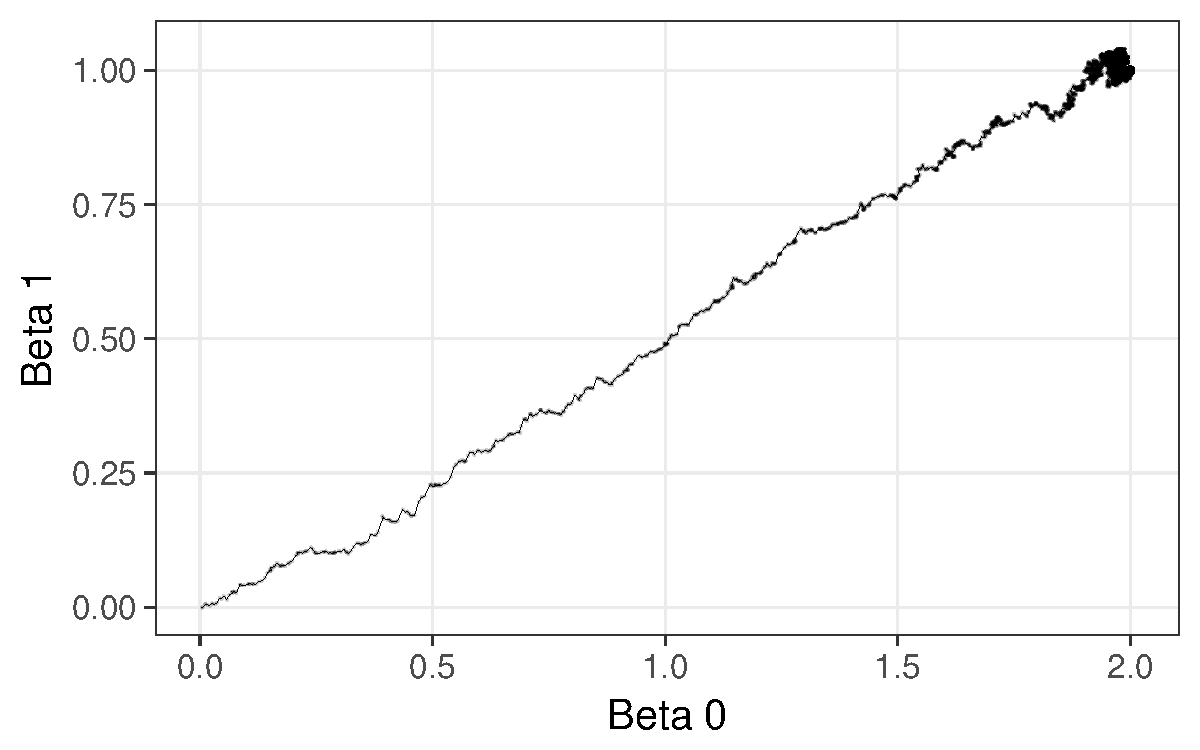
\includegraphics[width=0.9\textwidth]{lin_reg_example_1_SGD_iter_all.pdf}
  \caption{Iterations of stochastic gradient descent algorithm for linear regression.}
  \label{fig:lin_reg_example_1_SGD_iter_all}
\end{figure}

\begin{figure}[H]
  \centering
  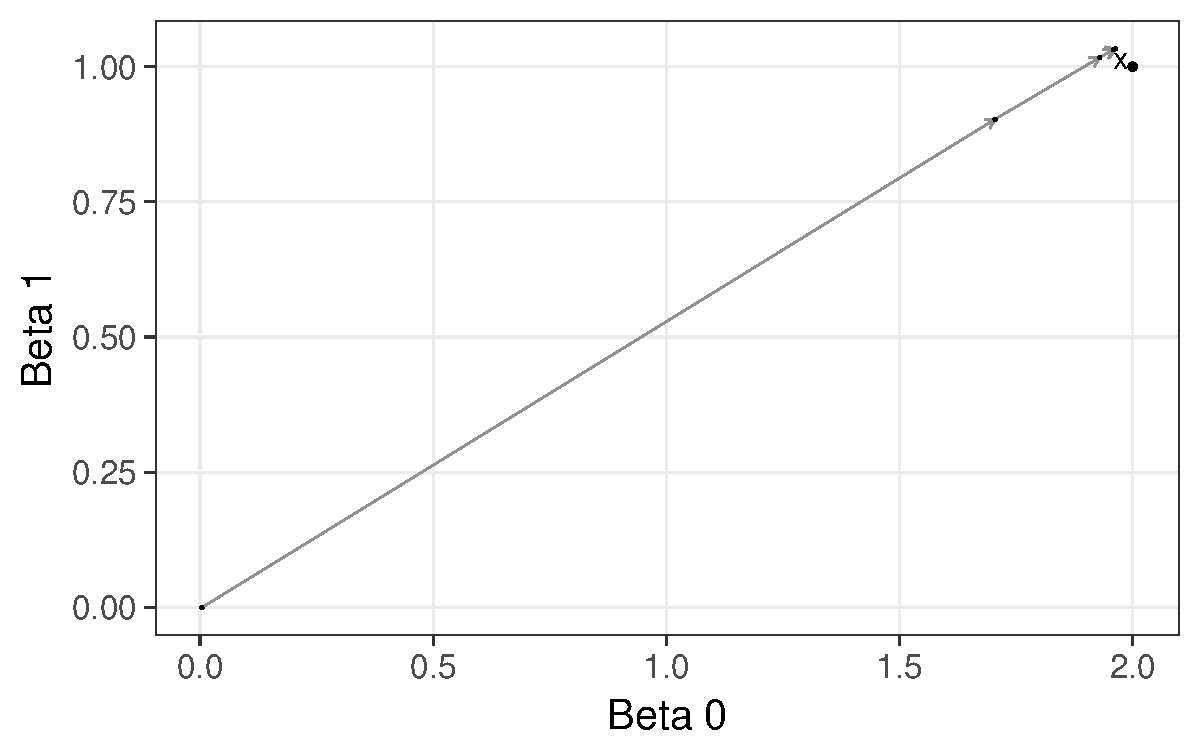
\includegraphics[width=0.9\textwidth]{lin_reg_example_1_SGD_each_epoch.pdf}
  \caption{Iterations of stochastic gradient descent algorithm for linear regression. Each arrow points to the value of the parameters after each epoch.}
  \label{fig:lin_reg_example_1_SGD_each_epoch}
\end{figure}


We can see that in the second figure that the directions go zigzagging, but in the end reach the final solution. In GD the directions were more uniform.

In both figures there's once more the big dot that represents the real value of the parameters ($\beta_0=2$ y $\beta_1 = 1$) and the x that represents the value from the \texttt{lm} package, but the second image isn't that clear because of all the noise in the directions.

\textbf{Logistic regression}

For logistic regression, each $\psi_i(x, \theta)$ is

$$
\psi_i(x, \theta) = y_i \log(h(\beta^T x_i)) + (1-y_i) \log(1-h(\beta^T x_i)) = \ell_i(x, \beta).
$$ 

And we can get to the following result

\[
\frac{\partial \ell_i}{\partial \beta_j} = \frac{\partial \psi_i}{\partial \beta_j} = x_{ij}(y_i - h(\beta^T x_i)).
\]

In the implementation, the stopping criteria was the same as in SGD for linear regression.

Figures \ref{fig:log_reg_example_1_SGD_iter_all} and \ref{fig:log_reg_example_1_SGD_each_epoch} show the values of the parameters in each iteration. As before, the first figure shows only the beginning of each epoch and the second shows all iterations in all epochs. The values converge to the real values and the values that we get if we use the \texttt{glm} package.

% ```{r, warning=FALSE}

% # Plots only at the beginning of each epoch
% plot_gd_iter(data_gradient_descent, model, beta_0, beta_1, 1)

% # Plots all iterations in all epochs
% data_gradient_descent %>% 
%   ggplot(aes(beta_0, beta_1)) +
%   xlab("Beta 0") +
%   ylab("Beta 1") +
%   geom_point(size = 0.01, color = 'black', alpha = 0.2) +
%   geom_point(aes(x, y),
%              data = tibble(x = beta_0,
%                            y = beta_1)) +
%   geom_point(aes(x, y),
%              data = tibble(x = model$coefficients[1],
%                            y = model$coefficients[2]),
%              shape = 'x',
%              size = 5) +
%   theme(
%     panel.grid.minor = element_blank()
%   )

% ```

\begin{figure}[H]
  \centering
  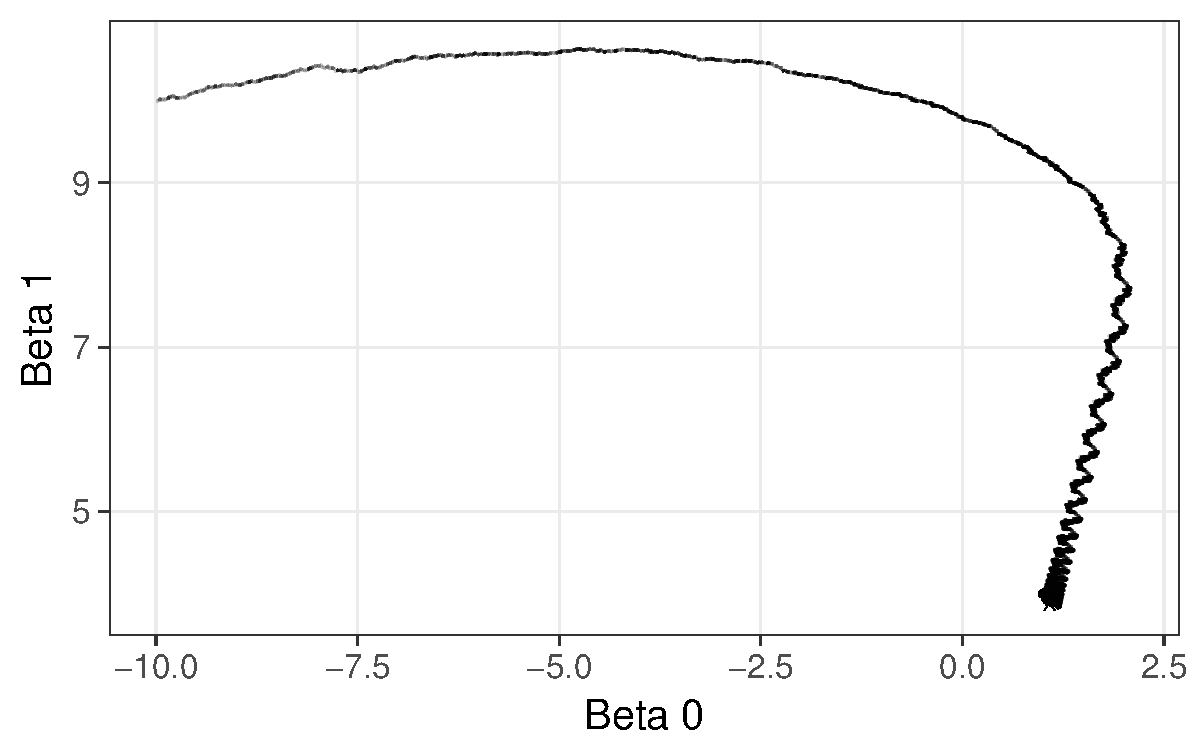
\includegraphics[width=0.9\textwidth]{log_reg_example_1_SGD_iter_all.pdf}
  \caption{Iterations of stochastic gradient descent algorithm for logistic regression.}
  \label{fig:log_reg_example_1_SGD_iter_all}
\end{figure}
